\chapter{Основные понятия и определения}
\selectlanguage{russian}

Изучение курса <<Защита информации>> необходимо начать с определения понятия \emph{<<информация>>}. В теоретической информатике \emph{информация} -- это любые сведения, или цифровые данные, или сообщения, или документы, или файлы, которые могут быть переданы \emph{получателю информации} от \emph{источника информации}. Можно считать, что информация передаётся по какому-либо каналу связи с помощью некоторого носителя, которым может быть, например, распечатка текста, диск или другое устройство хранения информации, система передачи сигналов по оптическим, проводным линиям или радиолиниям связи и~т.\,д.

\emph{Защита информации} -- это\footnote{Строго говоря, определение защиты информации даётся в официальном стандарте ГОСТ Р 50922-2006, <<Защита информации. Основные термины и определения>>~\cite{GOST-50922-2006}, согласно которому \emph{защита информации} -- это деятельность, направленная на предотвращение утечки защищаемой информации, несанкционированных и непреднамеренных воздействий на защищаемую информацию. Однако мы пользуемся определением, основанным на понятии <<безопасность информации>> из того же стандарта: \emph{безопасность информации} -- это состояние защищённости информации, при котором обеспечиваются ее \emph{конфиденциальность}, \emph{доступность} и \emph{целостность}.} обеспечение \emph{целостности}, \emph{конфиденциальности} и \emph{доступности} информации, передаваемой или хранимой в какой-либо форме. Информацию необходимо защищать от нарушения её целостности и конфиденциальности в результате вмешательства \emph{нелегального пользователя}. В российском стандарте ГОСТ Р 50.1.056-2005 приведены следующие определения~\cite{GOST-2005}:
\begin{itemize}
	\item \emph{целостность информации}\index{целостность} -- состояние информации, при котором отсутствует любое ее изменение, либо изменение осуществляется только преднамеренно субъектами, имеющими на него право;
	\item \emph{конфиденциальность}\index{конфиденциальность} -- состояние информации, при котором доступ к ней осуществляют только субъекты, имеющие на него право;
	\item \emph{доступность}\index{доступность} -- состояние информации, при котором субъекты, имеющие права доступа, могут реализовать их беспрепятственно.
\end{itemize}

Другой стандарт ГОСТ Р ИСО/МЭК 13335-1-2006~\cite{GOST-13335-1-2006} определяет \emph{информационную безопасность} как все аспекты, связанные с определением, достижением и поддержанием \emph{конфиденциальности}, \emph{целостности}, \emph{доступности}, \emph{неотказуемости}, \emph{подотчётности}, \emph{аутентичности} и \emph{достоверности} информации или средств ее обработки. То есть в дополнение к предыдущему определению, на защиту информации в области информационных технологий возлагаются дополнительные задачи:
\begin{itemize}
	\item обеспечение \emph{неотказуемости} -- способность удостоверять имевшие место действия или события так, чтобы эти события или действия не могли быть позже отвергнуты;
	\item обеспечение \emph{подотчётности} -- способность однозначно прослеживать действия любого логического объекта;
	\item обеспечение \emph{аутентичности} -- способность гарантировать, что субъект или ресурс идентичны заявленным;\footnote{Аутентичность применяется к таким субъектам, как пользователи, к процессам, системам и информации.}
	\item обеспечение \emph{достоверности} -- способность обеспечивать соответствие предусмотренному поведению и результатам.
\end{itemize}

Стандарт ГОСТ Р 50922-2006~\cite{GOST-50922-2006}, хотя и не вводит прямой классификации методов защиты информации, даёт следующие их определения.
\begin{itemize}
	\item \emph{Правовая защита информации}. Защита информации правовыми методами, включающая в себя разработку законодательных и нормативных правовых документов (актов), регулирующих отношения субъектов по защите информации, применение этих документов (актов), а также надзор и контроль за их исполнением.
	\item \emph{Техническая защита информации; ТЗИ}. Защита информации, заключающаяся в обеспечении некриптографическими методами безопасности информации (данных), подлежащей (подлежащих) защите в соответствии с действующим законодательством, с применением технических, программных и программно-технических средств.
	\item \emph{Криптографическая защита информации}. Защита информации с помощью её криптографического преобразования.
	\item \emph{Физическая защита информации}. Защита информации путём применения организационных мероприятий и совокупности средств, создающих препятствия для проникновения или доступа неуполномоченных физических лиц к объекту защиты.
\end{itemize}

В рамках данного пособия в основном остановимся на криптографических методах защиты информации. Они помогают обеспечить \emph{конфиденциальность} и \emph{аутентичность}. В сочетании с правовыми методами защиты информации они помогают обеспечить \emph{неотказуемость} действий, а в сочетании с техническими -- \emph{целостность информации} и \emph{достоверность}.

При изучении криптографических методов защиты информации используются дополнительные определения. В целом науку о создании, анализе и использовании криптографических методов называют \emph{криптологией}. Её разделяют на \emph{криптографию}, посвящённую разработке и применению криптографических методов, и \emph{криптоанализ}, который занимается поиском уязвимостей в существующих методах. Данное разделение на криптографию и криптоанализ (и, соответственно, разделение на \emph{криптографов} и \emph{криптоаналитиков}) условно, так как создать хороший криптографический метод невозможно без умения анализировать его потенциальные уязвимости, а поиск уязвимостей в современных криптографических методах нельзя осуществить без знания методов их построения.

Попытка криптоаналитика нарушить свойство криптографической системы по обеспечению защиты информации (например, получить информацию вопреки свойству обеспечения конфиденциальности) называется \emph{криптографической атакой} (\emph{криптоатакой}). Если данная попытка оказалась успешной, и свойство было нарушено или может быть нарушено в ближайшем будущем, то такое событие называется \emph{взломом криптосистемы} или \emph{вскрытием криптосистемы}. Конкретный метод криптографической атаки также называется \emph{криптоанализом} (например, линейный криптоанализ, дифференциальный криптоанализ и~т.~д.). Криптосистема называется \emph{криптостойкой}, если число стандартных операций для её взлома превышает возможности современных вычислительных средств в течение всего времени ценности информации (до 100 лет).

Для многих криптографических примитивов существует атака полным перебором\index{атака!полным перебором} или аналогичная, которая подразумевает, что если выполнить очень большое количество определённых операций (по одной на каждое значение из области определения одного из аргументов криптографического метода), то один из результатов укажет непосредственно на способ взлома системы (например, укажет на ключ для нарушения конфиденциальности, обеспечиваемой алгоритмом шифрования, или на допустимый прообраз для функции хеширования, приводящий к нарушению аутентичности и целостности). В этом случае под \emph{взломом криптосистемы} понимается построение алгоритма криптоатаки с количеством операций меньшим, чем планировалось при создании этой криптосистемы (часто, но не всегда, это равно именно количеству операций при атаке полным перебором\footnote{Например, сложность построения второго прообраза для хеш-функций на основе конструкции Меркла~---~Дамгарда составляет $2^n / \left|M\right|$ операций, тогда как полный перебор -- $2^n$. См. раздел~\ref{section-stribog}.}). Взлом криптосистемы -- это не обязательно, например, реально осуществлённое извлечение информации, так как количество операций может быть вычислительно недостижимым как в настоящее время, так и в течение всего времени защиты. То есть могут существовать системы, которые формально взломаны, но пока ещё являются криптостойкими.

Далее рассмотрим модель передачи информации с отдельными криптографическими методами.

\section[Модели систем передачи информации]{Модели систем передачи информации с криптографической защитой}\index{канал связи!защищённый|(}\index{канал связи!открытый|(}
\selectlanguage{russian}

Простая модель системы передачи с криптографической защитой представлена на рис.~\ref{pic:model-simple}. На рисунке показаны легальный отправитель, легальный получатель и криптоаналитик, который пытается нарушить безопасность информации в системе. Данные в системе передаются по открытому каналу связи. Можно также говорить, что криптографические преобразования на стороне отправителя и получателя позволили им создать \emph{защищённый канал связи} поверх открытого канала, как показано на рис.~\ref{pic:model-simple-with-channel}.

\begin{figure}[!thb]
	\centering
	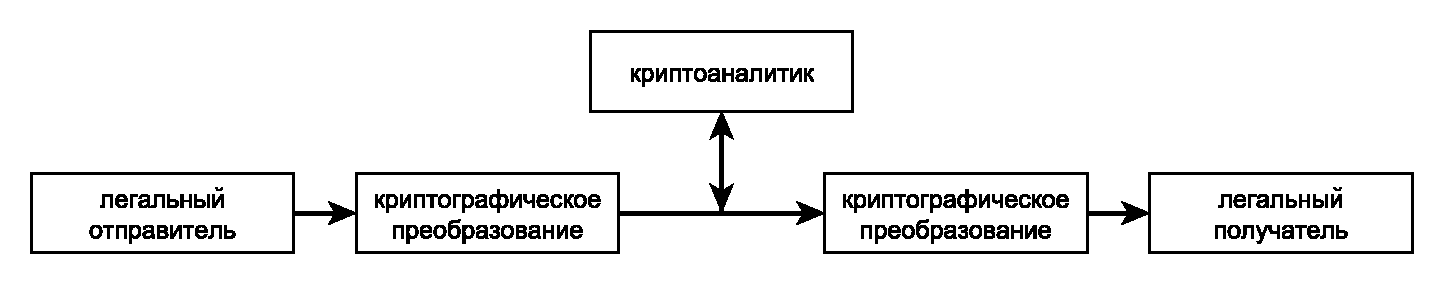
\includegraphics[width=1.0\textwidth]{pic/model-simple}
	\caption{Модель системы передачи информации с криптографической защитой по открытому каналу\label{pic:model-simple}}
\end{figure}

\begin{figure}[!thb]
	\centering
	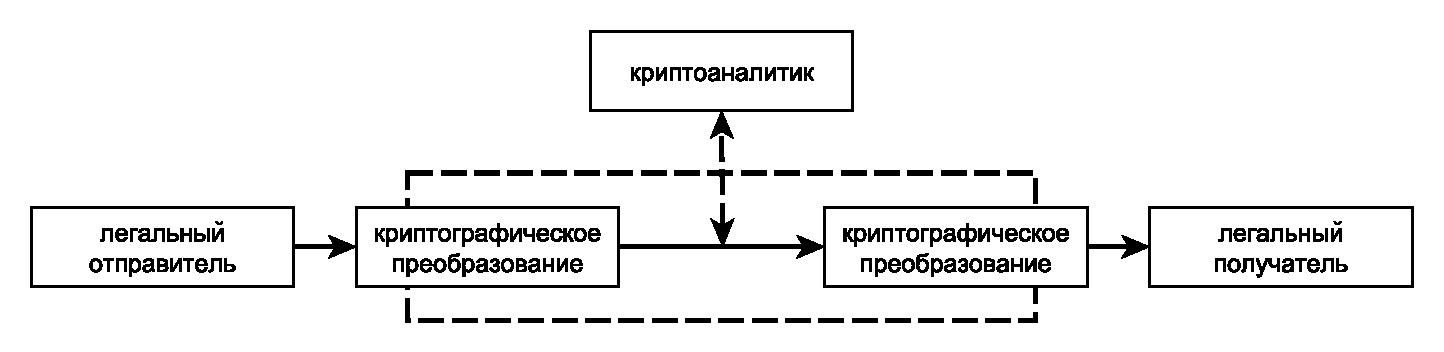
\includegraphics[width=1.0\textwidth]{pic/model-simple-with-channel}
	\caption{Открытый и защищённый каналы связи в модели системы передачи информации с криптографической защитой\label{pic:model-simple-with-channel}}
\end{figure}

Для обеспечения конфиденциальности информации используются криптографические системы с функцией шифрования. Пример системы с шифрованием показан на рис.~\ref{pic:model-cipher}.

\begin{figure}[!thb]
	\centering
	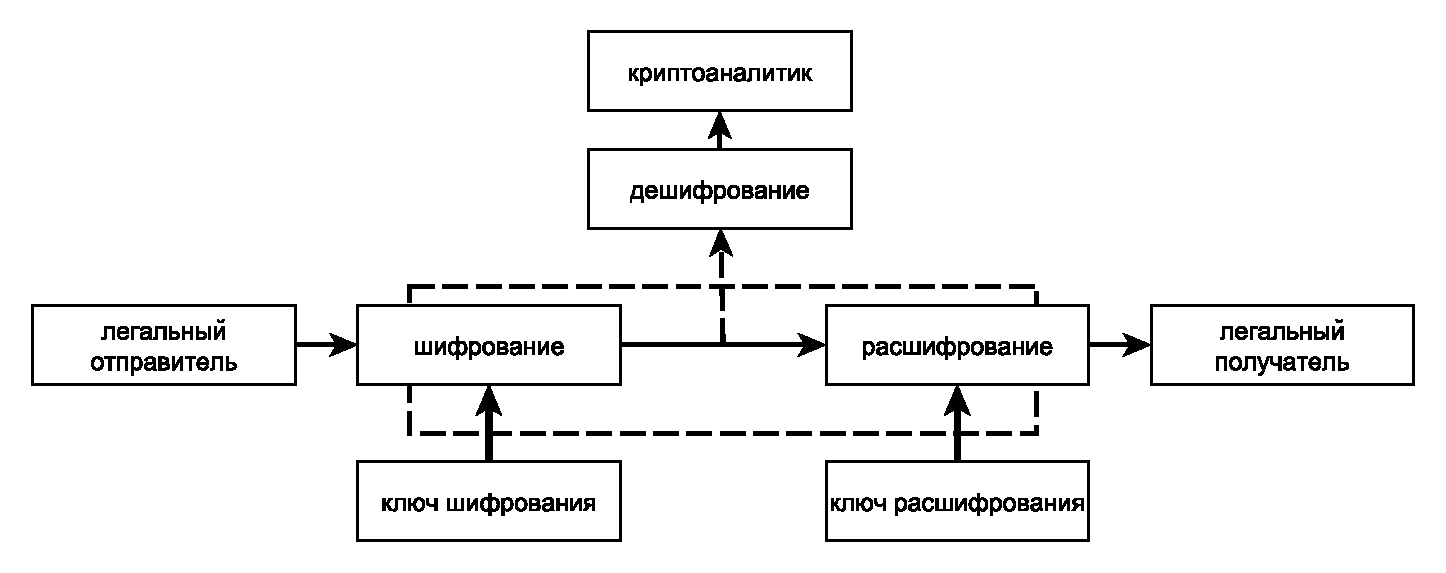
\includegraphics[width=1.0\textwidth]{pic/model-cipher}
	\caption{Модель системы передачи информации с шифрованием\label{pic:model-cipher}}
\end{figure}

Легальный отправитель \emph{шифрует} (\langen{cipher}) сообщение (\emph{открытый текст}\index{открытый текст}, \langen{plaintext}) с использованием \emph{ключа шифрования}\index{ключ!шифрования} (\langen{encryption key}) и передаёт зашифрованное сообщение (\emph{шифртекст}\index{шифртекст}, \langen{ciphertext, cyphertext} или \emph{шифрограмма}\index{шифрограмма}\footnote{Строго говоря, \emph{шифрограмма} -- это \emph{шифртекст} после его \emph{кодирования} для целей передачи по каналу связи.}) по открытому каналу связи. Легальный получатель \emph{расшифровывает} сообщение, используя \emph{ключ расшифрования}\index{ключ!расшифрования}, в общем случае отличающийся от ключа шифрования. Нелегальный пользователь, называемый криптоаналитиком, пытается \emph{дешифровать}\footnote{Обратите внимание, что в англоязычной литературе словом <<\textit{decryption}>> обозначается и расшифрование, и дешифрование.} сообщение, не имея ключа расшифрования, то есть нарушить конфиденциальность передаваемой информации. Можно сказать, что функции шифрования и расшифрования вместе с конкретными ключами шифрования и расшифрования помогли легальным участникам системы установить защищённый канал связи, обеспечивающий конфиденциальность информации.

\emph{Шифрование} (\emph{зашифрование}) -- это обратимое преобразование данных, формирующее шифртекст из открытого текста. \emph{Расшифрование} -- операция, обратная шифрованию. А вместе это \emph{шифр} -- криптографический метод, используемый для обеспечения конфиденциальности данных, включающий алгоритм зашифрования и алгоритм расшифрования.~\cite{GOST-89}

\emph{Шифр}\index{шифр} -- это множество обратимых функций отображения $E_{K_1}$\index{функция!шифрования} множества открытых текстов $\set{M}$ на множество шифртекстов $\set{C}$, зависящих от выбранного ключа шифрования $K_1$ из множества $\set{K}_E$, а также соответствующие им обратные функции расшифрования $D_{K_2}$, $\set{K}_D$, отображающие множество шифртекстов на множество открытых текстов:
\begin{equation}\label{eq:Encryption}\begin{array}{l}
	E_{k_1}, k_1 \in \set{K}_E: \set{M} \to \set{C}, \\
	D_{k_2}, k_2 \in \set{K}_D: \set{C} \to \set{M}, \\
	\forall k_1 \in \set{K}_E ~ \exists k_2 \in \set{K}_D: \\
	\forall m \in \set{M}: ~ E_{k_1} \left( m \right) = c, c \in \set{C}: \\
	D_{k_2} \left( c \right) = m.
\end{array}\end{equation}

Можно сказать, что шифрование -- это обратимая функция двух аргументов: сообщения и ключа. Обратимость -- основное условие корректности шифрования, по которому каждому зашифрованному сообщению $Y$ и ключу $K$ соответствует одно исходное сообщение $X$. Легальный пользователь $B$ (на приёмной стороне системы связи) получает сообщение $Y$ и осуществляет процедуру \emph{расшифрования}\index{расшифрование}.

Следует отличать \emph{шифрование} от \emph{кодирования}, будь то кодирование источника или канала. Под кодированием источника понимается преобразование информации для более компактного хранения, а под кодированием канала -- для повышения помехоустойчивости.

Модель системы передачи информации с обеспечением аутентичности передаваемых сообщений выглядит, как показано на рис.~\ref{pic:model-auten}.

\begin{figure}[!thb]
	\centering
	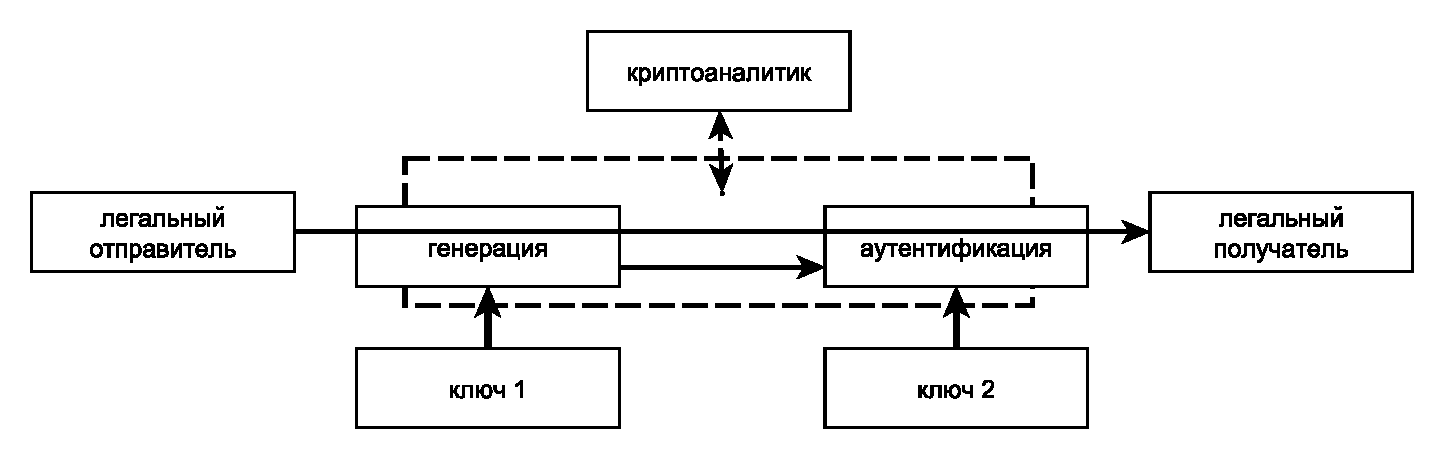
\includegraphics[width=1.0\textwidth]{pic/model-auten}
	\caption{Модель системы передачи информации с обеспечением аутентичности передаваемых сообщений\label{pic:model-auten}}
\end{figure}

В этой модели сообщение передаётся по открытому каналу связи без изменений (в открытом виде), однако вместе с сообщением от легального пользователя по тому же каналу связи передаётся дополнительная информация. Специальные криптографические методы позволяют гарантировать, что данную информацию может сформировать только легальный пользователь (или, в некоторых случаях, ещё и легальный получатель). Легальный получатель проверяет эту дополнительную информацию и убеждается, что сообщение пришло именно от легального отправителя и без изменений. Таким образом был организован защищённый канал связи с обеспечением аутентичности передаваемых сообщений. 

\index{канал связи!защищённый|)}\index{канал связи!открытый|)}


\section[Классификация]{Классификация криптографических механизмов}

\subsection{Симметричные и асимметричные криптосистемы}
\selectlanguage{russian}

Криптографические системы и шифры можно разделить на две большие группы в зависимости от принципа использования ключей для шифрования и расшифрования.

Если для шифрования и расшифрования используется один и тот же ключ $K$, либо если получение ключа расшифрования $K_2$ из ключа шифрования $K_1$ является тривиальной операцией, то такая криптосистема называется \emph{симметричной}\index{криптосистема!симметричная}. В зависимости от объёма данных, обрабатываемых за одну операцию шифрования, симметричные шифры делятся на \emph{блочные}\index{шифр!блочный}, в которых за одну операцию шифрования происходит преобразование одного блока данных (32 бита, 64, 128 или больше), и \emph{потоковые}\index{шифр!потоковый}, в которых работают с каждым символом открытого текста по отдельности (например, с 1 битом или 1 байтом). Примеры блочных шифров рассмотрены в главе~\ref{chapter-block-ciphers}, а потоковых -- в главе~\ref{chapter-stream-ciphers}.

Использование блочного шифра подразумевает разделение открытого текста на блоки одинаковой длины, к каждому из которых применяется функция шифрования. Кроме того, результат шифрования следующего блока может зависеть от предыдущего\footnote{Строго говоря, функция шифрования может применяться не только к самому блоку данных, но и к другим параметрам текущего отрывка открытого текста. Например, к его позиции в тексте (\langen{offset}) или даже к результату шифрования предыдущего блока.}. Данная возможность регулируется \emph{режимом работы блочного шифра}. Примеры нескольких таких режимов рассмотрены в разделе~\ref{section-block-chaining}.

Если ключ расшифрования получить из ключа шифрования вычислительно сложно, то такие криптосистемы называют криптосистемами \emph{с открытым ключом}\index{криптосистема!с открытым ключом} или \emph{асимметричными} криптосистемами\index{криптосистема!асимметричная}. Некоторые из них рассмотрены в главе~\ref{chapter-public-key}. Все используемые на сегодняшний день асимметричные криптосистемы работают с открытым текстом, составляющим несколько сотен или тысяч бит, поэтому классификация таких систем по объёму обрабатываемых за одну операцию данных не производится.

Алгоритм, который выполняет отображение аргумента произвольной длины в значение фиксированной длины, называется \emph{хеш-функцией}. Если для такой хеш-функции выполняются определённые свойства, например, устойчивость к поиску коллизий, то это уже \emph{криптографическая хеш-функция}. Такие функции рассмотрены в главе~\ref{chapter-hash-functions}.

Для проверки аутентичности сообщения с использованием общего секретного ключа отправителем и получателем используется \emph{код аутентификации [сообщения]} (другое название в русскоязычной литературе - \emph{имитовставка}, \langen{message authentication code, MAC}), рассмотренный в разделе~\ref{section-MAC}. Его аналогом в криптосистемах с открытым ключом является \emph{электронная подпись}, алгоритмы генерации и проверки которой рассмотрены в главе~\ref{chapter-public-key} вместе с алгоритмами асимметричного шифрования.

\subsection{Шифры замены и перестановки}

Шифры по способу преобразования открытого текста в шифртекст разделяются на шифры замены и шифры перестановки.

\input{substitution_ciphers}

\input{permutation_ciphers}

\input{composite_ciphers}

\subsection{Примеры современных криптографических примитивов}

Приведём примеры названий некоторых современных криптографических примитивов, из которых строят системы защиты информации.
\begin{itemize}
    \item DES\index{шифр!DES}, AES, ГОСТ 28147-89, Blowfish\index{шифр!Blowfish}, RC5\index{шифр!RC5}, RC6\index{шифр!RC6} -- блочные симметричные шифры, скорость обработки -- десятки мегабайт в секунду.
    \item A5/1, A5/2, A5/3\index{шифр!A5}, RC4\index{шифр!RC4} -- потоковые симметричные шифры с высокой скоростью. Семейство A5 применяется в мобильной связи GSM, RC4 -- в компьютерных сетях для SSL-соединения между браузером и веб-сервером.
    \item RSA\index{шифр!RSA} -- криптосистема с открытым ключом для шифрования.
    \item RSA\index{электронная подпись!RSA}, DSA\index{электронная подпись!DSA}, ГОСТ Р 34.10-2001\index{электронная подпись!ГОСТ Р 34.10-2001} -- криптосистемы с открытым ключом для электронной подписи.
    \item MD5\index{хеш-функция!MD5}, SHA-1\index{хеш-функция!SHA-1}, SHA-2\index{хеш-функция!SHA-2}, ГОСТ Р 34.11-94\index{хеш-функция!ГОСТ Р 34.11-94} -- криптографические хеш-функции.
\end{itemize}

\section{Методы криптоанализа и типы атак}
\selectlanguage{russian}

Нелегальный пользователь-криптоаналитик получает информацию путём дешифрования. Сложность этой процедуры определяется числом стандартных операций, которые надо выполнить для достижения цели. \emph{Двоичной сложностью}\index{сложность!двоичная} (или битовой сложностью) алгоритма называется количество двоичных операций, которые необходимо выполнить для его завершения.

Рассмотрим основные сценарии работы криптоаналитика $E$. В первом сценарии криптоаналитик может осуществлять подслушивание и (или) перехват сообщений. Его вмешательство не нарушает целостности информации: $Y=\widetilde{Y}$, где Y -- информация, как случайная величина, до вмешательства, $\widetilde{Y}$ -- после вмешательства. Эта роль криптоаналитика называется \emph{пассивной}. Так как он получает доступ к информации, то здесь нарушается конфиденциальность.

Во втором сценарии роль криптоаналитика \emph{активная}. Он может подслушивать, перехватывать сообщения и преобразовывать их по своему усмотрению: задерживать, искажать с помощью перестановок пакетов, устраивать обрыв связи, создавать новые сообщения и т.~п. В этом случае выполняется условие $Y \neq \widetilde{Y}$. Это значит, что одновременно нарушается целостность и конфиденциальность передаваемой информации.

Приведём примеры пассивных и активных атак:
\begin{itemize}
    \item Атака <<человек посередине>>\index{атака!<<человек посередине>>} (\langen{man-in-the-middle}) подразумевает криптоаналитика, который разрывает канал связи, встраиваясь между $A$ и $B$, получает сообщения от $A$ и от $B$, а от себя отправляет новые, фальсифицированные сообщения. В результате $A$ и $B$ не замечают, что общаются с $E$, а не друг с другом.
    \item Атака \emph{воспроизведения}\index{атака!воспроизведения} (\langen{replay attack}) предполагает, что криптоаналитик может записывать и воспроизводить шифртексты, имитируя легального пользователя.
    \item Атака на \emph{различение} сообщений\index{атака!на различение} означает, что криптоаналитик, наблюдая одинаковые шифртексты, может извлечь информацию об идентичности исходных открытых текстов.
    \item Атака на \emph{расширение} сообщений\index{атака!на расширение} означает, что криптоаналитик может дополнить шифртекст осмысленной информацией без знания секретного ключа.
    \item \emph{Фальсификация} шифртекстов\index{атака!фальсификацией} криптоаналитиком без знания секретного ключа.
\end{itemize}

Часто для нахождения секретного ключа криптоатаки строят в предположениях о доступности дополнительной информации. Приведём примеры:
\begin{itemize}
    \item Атака на основе известного открытого текста\index{атака!с известным открытым текстом} (\langen{chosen plaintext attack, CPA}) предполагает, что криптоаналитик имеет возможность выбирать открытый текст и получать для него соответствующий шифртекст.
    \item Атака на основе известного шифртекста\index{атака!с известным шифртекстом} (\langen{chosen ciphertext attack, CCA}) предполагает возможность криптоаналитику выбирать шифртекст и получать для него соответствующий открытый текст.
\end{itemize}

Обязательным требованием к современным криптосистемам является устойчивость ко всем известным типам атак: пассивным, активным и с дополнительной информацией.


%Приведём примеры возможных вариантов работы активного криптоаналитика.
%\begin{itemize}
%\item Криптоаналитик имеет $m$ шифрованных сообщений $Y_{1},Y_{2},\ldots Y_{m}$ и пытается определить ключ или прочитать открытый текст $X_{1},X_{2},\ldots X_{m}.$
%\item Криптоаналитик имеет несколько пар открытого и шифрованного текстов
%
%$(Y_{1},X_{1}),(Y_{2}X_{2}),\ldots (Y_{m}X_{m})$ и пытается дешифровать остальной текст или определить алгоритм шифрования или определить ключ.
%\item
%\item
%\item
%\end{itemize}

Для защиты информации от активного криптоаналитика и обеспечения её целостности дополнительно к шифрованию сообщений применяют имитовставку\index{имитовставка}. Для неё используют обозначение $\MAC$ (\langen{message authentication code}). Как правило, $\MAC$ строится на основе хеш-функций, которые будут описаны далее.

Существуют ситуации, когда пользователи $A$ и $B$ не доверяют друг другу. Например, $A$ -- банк, $B$ -- получатель денег. $A$ утверждает, что деньги были переведены, $B$ - что перевода не было. Решение задачи аутентификации и неотрицаемости состоит в обеспечении \emph{электронной подписью}\index{электронная подпись} каждого из абонентов. Предварительно надо решить задачу о генерировании и распределении секретных ключей.

В общем случае системы защиты информации должны обеспечивать:
\begin{itemize}
    \item конфиденциальность\index{конфиденциальность} (защиту от наблюдения),
    \item целостность\index{целостность} (защиту от изменения),
    \item аутентификацию (защиту от фальсификации пользователя и сообщений),
    \item доказательство авторства информации (доказательство авторства и защита от его отрицания)
\end{itemize}
как со стороны получателя, так и со стороны отправителя.

Важным критерием для выбора степени защиты является сравнение стоимости реализации взлома для получения информации и экономического эффекта от владения ей. Очевидно, что если стоимость взлома превышает ценность информации, взлом нецелесообразен.

%Сценарии защиты информации
%   Сценарий 1. A -- передающая сторона. B -- принимающая сторона. E -- пассивный
%криптоаналитик, который может подслушивать передачу, но не может вмешиваться
%в процесс передачи. Цель защиты: обеспечение конфиденциальности. Средства
%-- методы шифрования с секретным ключом (симметричные системы шифрования)
%и методы шифрования с открытым ключом (асимметричные системы шифрования).
%Сценарий 2. E -- активный криптоаналитик, который может изменять, удалять и вставлять
%сообщения или их части. Цель защиты -- обеспечение конфиденциальности (не
%всегда) и обеспечение целостности. Средства -- методы шифрования и добавление
%имитовставки\index{имитовставка} (Message Authentication Code -- $\MAC$).
%Сценарий 3. A и B не доверяют друг другу. Цель защиты -- аутентификация пользователя.
%Средства -- электронная подпись.


\input{The_minimum_key_lengths}
